\chapter{Contribution}

This chapter is divided into multiple sections, which cover the architecture and the expandability of the implementation. The architecture is split into subsections covering the various components that were implemented throughout the thesis. Overall it should give the reader an understanding of the motivation and decisions done to implement the requirements.

%Most important chapter of the thesis. Describes what the author contributes as research. Discusses intuition, motivation, describes and reasons about necessity of proposed elements. Defines theses based on reasonable assumptions. Discusses relevant aspects of contribution. Approximately 30 to 40 pages. Can be split into multiple chapters.

\section{Architecture}

The architecture is in the most classical way a microservice orientated architecture. Compared to a monolithic application there is a higher focus on single components and their implementation and therefore decouple the complexity in its entirety.

Services itself can be clustered into the "Distributed Crawler", "Distributed Analysis", "Database", and "Frontend" sections, whereas the database is a third party implementation that is built upon and integrated into the architecture. The visualization of the microservice architecture can be seen in \ref{fig:architecture}.

\todo{redo image with clustered sections}
\begin{figure}[H]
    \centering
    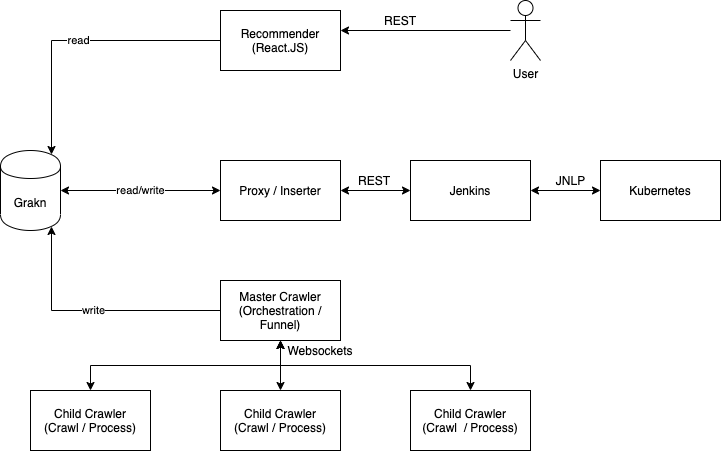
\includegraphics[scale=0.5]{graphics/architecture_v2.png}
    \caption{Architectural representation of the system as a whole}
    \label{fig:architecture}
\end{figure}

\subsection{Database - Grakn.ai}
One of the fundamental decisions is which database to select as a lot of other components will have to build upon it. From the beginning on it was clear that for building a knowledge graph some sort of graph database could be utilized as it will clearly show the relations of all entities and help in building a recommender system due to the sheer amount of data in the graph.
The implementation could have been done with a NoSQL or a classical SQL database as well, but would have required more linking of data to represent the same sort of result using a graph database.

The first candidate for a graph database that comes to mind is neo4j\footnote{https://neo4j.com}, which is one of the older ones publicly released in 2007\todo{quote https://neo4j.com/developer/graph-database/\#neo4j-overview}. While neo4j could have been used for the implementation, it felt quite outdated when it came to the data representation and their query language "Cypher". Therefore the graph database Grakn\footnote{https://grakn.ai} was used, which was released in 2016\todo{quote source }.

Grakn describes itself as a knowledge graph engine to organize complex networks of data and making it queryable, by performing knowledge engineering\todo{quote https://grakn.ai/grakn-core}. It fully supports the Entity-Relationship model and comes along with a query language called Graql. 

\todo{Deduplication}
\subsubsection{Entity-Relationship model}
Entity-Relationship models are the de facto standard to represent a schema for a graph database.
\todo{redo er model}
\begin{figure}[H]
    \centering
    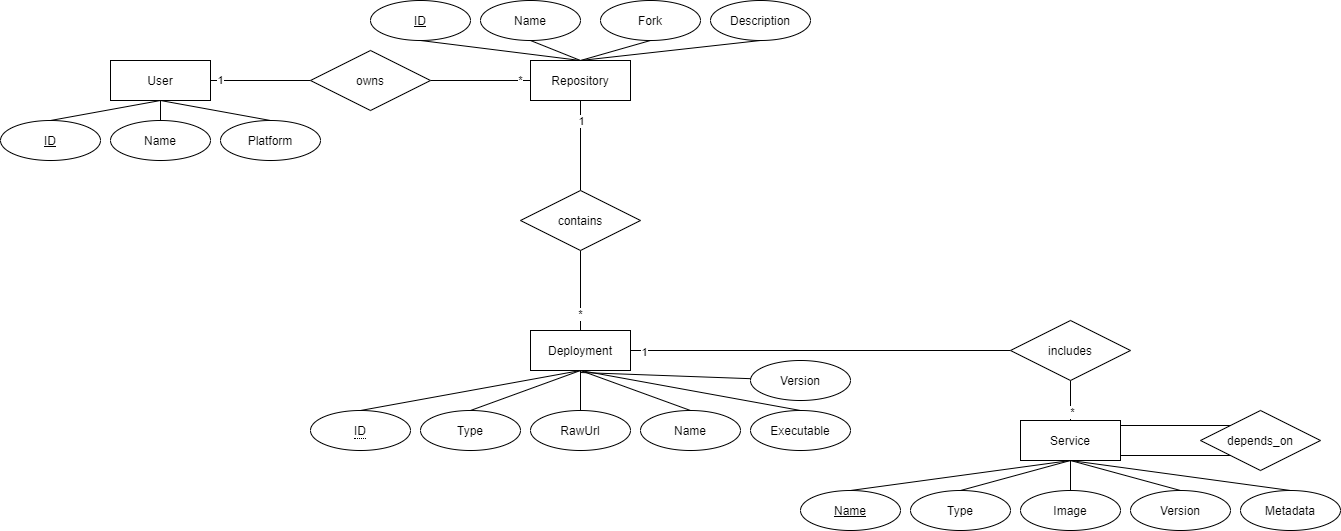
\includegraphics[width=1.2\paperwidth,height=1.2\paperheight,keepaspectratio,angle=270]{graphics/er_database.png}
    \caption{Entity-Relationship model}
    \label{fig:er_model}
\end{figure}

Deployment Scripts do not follow a standard and therefore a generalized model has to be created that possibly fit most of them. The focus was lying on the deployment as this entity represents the script itself as a whole. Followed by services that are defined in the deployment script and therefore have a direct relationship to the deployment. Services can occur unlimited times in a deployment, but one service can always only have one deployment. This was kept this way as services, depending on the context you are in, can be differently defined when it comes to versions or extra attributes, but as we are dealing with a graph database searching for possibly best fits will still work easy as one has the direct relationship between services and its deployment.
Services can depend on itself as well, meaning that those are more coupled than others, e.g. a database and a backend for example. Once more this depends highly on the context one is in and will be part of another section in this chapter. \todo{e.g. kustomize, kuberentes, helm, docker-compose fit this schema}
As the deployment script is usually embedded in a repository a coupling is happening there as well. The repository could represent in a classical way a repository on either GitHub or Bitbucket, but could also be a website or documentation depending on where it was found. One repository can hold an unlimited amount of deployment scripts and one can possibly belong to multiple repositories. The simple explanation is that the secure hash algorithm is used as key identification and files that have the same content will therefore have relationships added to those repositories as well, while still keeping only one deployment entity in the database. The last entity in the schema is a user that owns unlimited repositories, while one repository can only belong to one user.

One of the favorable aspects of Grakn is how it handles duplicates. As long as one defines unique keys in the attributes of an entity there will not be a duplicate as those will automatically be dropped on insertion. This will keep the database free from duplicates and allows one to concentrate on the actual implementation of their use case.

The schema is kept general in regards to the domain of different kinds of deployment scripts while overall favouring the origin from code repositories. A visualization of the schema can be seen in figure \ref{fig:er_model} and gives a self explanatory overview according to current standards in ER models.

Grakn supports the feature of having an attribute as a key attribute and therefore providing uniqueness across one entity based on this key. While Grakn provides its own internal ID it was usefull and necessary to give each entity and relation a self defined key attribute to not have an additional mapping of Grakn ID to e.g. GitHub IDs or other elements to uniquely identify one relation or entity.

\subsubsection{Open Source Contributions}
Grakn is still quite a new graph database due to which the community around it is still rather small and problems that have been solved for others still have to covered for this one. Therefore some contributions to the project around Grakn and its tools have been covered in the implementation of this thesis.

First of all Grakn comes along with a tool called workbase, which is essentially an editor to show and edit the graph that the database contains. This is sufficient for most projects where the graph is rather small. The workbase is a Vue/React application wrapped in electron, which is a framework to create desktop applications from JavaScript. Therefore electron is wrapping the files with chromium and node.js to display the application cross platform. The workbase comes along with some flaws as graphs with nodes and edges in the 100.000 area will crash the application due to the limited amount of memory assigned to the chromium process and even in the area of 10.000 and more the application starts to stutter under the heavy load.

Therefore the first contribution in the domain of Grakn is a converter from Grakn to the the Graph Exchange XML Format (GEXF), which is essentially a file format to describe complex networks structures.
The advantage of GEXF is that it is an open specification and therefore implemented and used by a variation of applications and tools. One of these tools is Gephi, the open graph viz platform that allows to visualize and analyse networks of sizes in the area of multiple million nodes and edges. Another tool is the NetworkX\footnote{https://networkx.org/} framework for python, which allows to load and write GEXF files and therefore analyse networks further in the python universe.

The Grakn to GEXF converter reads a provided Grakn schema and generates proper queries for each entity and relation, followed by querying the database for the results and writing the results to a valid GEXF file, which in return can be further used by the tools mentioned earlier. Overall this will help to further analyse the graph as Grakn itself does not provide any tools for layouting, clustering coefficient, community detection and other metrics that might be interesting to extract out of a graph.

Another open source contribution was done in the direction of cloud compatibility as the open source version of the database does not come along with e.g. a helm chart or in general kubernetes manifests to deploy and seed a database one has to build the compatibility themselves. Important to know that the Grakn database is split between a server component and a console (cli) component, which are bundled into one docker image, while this makes it easier to e.g. debug the database it is not suitable to run as a sidecar container, as one simple does not the server component and even then one might run into the problem of seeding the database. The database can only be seeded if it is running, which makes kubernetes init containers useless as those will run before the actual container is running, therefore a sidecar is needed, meaning an additional container in the same pod to seed the database as soon as the server container is up and running. While this sounds relatively easy the Grakn console nor server provide a health point to check whether the database is really running, yes one can probe the port of the database but this will not guarantee that the database is really ready to receive connections. Therefore the second contribution is a sidecar container, containing a slim alpine image with the Grakn console and a startup script to check for the database to receive connections and if needed seed the database with a schema that can be mounted into the container.
One of the important points of infrastructure as code is reproducibility, meaning if one runs the code on different systems it should still result in the same end product, thus a manual seeding of the database would not be suitable.

\subsection{Distributed Crawler}
First and foremost the main part of the implementation is the so-called "distributed crawler", which follows the master and node pattern, where one entity is the master that controls the spawned nodes. In this thesis, it can also be seen as orchestrator/information funnel and the crawling/processing unit. The reason for calling it a distributed crawler is that the overall function of this implementation can be seen as a crawler and distributed in the sense that the nodes can be distributed across multiple data centers or even be used on edge nodes with the appropriate implementation.

The implementation was done using Node.js, which is an asynchronous JavaScript runtime, which allows to run JavaScript outside of the browser and potentially build scalable applications. One of the big advantages of Node.js is that you can use the synergies of running JavaScript on the server-side and client-side. While this might not be the first thing that comes to mind when thinking about a distributed crawler, it does come in handy as a lot of services offer an API\footnote{Application Programming Interface} that returns JSON\footnote{JavaScript Object Notation} objects. Those JSON objects are easier to deal with in its native environment compared to other programming languages where one would rely on a third party implementation and a lot of serialization as the implementation was simply not meant for that environment.
As JavaScript runs in a JavaScript engine, the V8 engine developed by Google, it can be extended by creating C++ modules to make certain functions quicker as those would natively run on the system.

The master and crawler nodes are all based on one unified code base and the only difference between the two is the addition of the database connection and the orchestration routes, which are both parts of the master node. The default startup parameter for a node is to act as a crawler and connect to the master, which can be changed by setting one environment variable called "TYPE" to "master". The node would therefore load the database module, orchestration routes and use the master implementation of the communication channel instead of the crawler one.
The benefits of a unified code base are that the application could be extended in the future to support e.g. leader election or let the master act as a crawler as well. Meaning depending on the processing power provided the master could handle on top of its own capabilities the ones of a crawler as well and therefore provide more coverage of crawled sources.
Leader election quickly explained is that e.g. 4 spawned crawler would elect one of their own to be the master node, which often works based on either first come first serves basis or other defined constraints.

Master and node in itself are on a fundamental level just web servers providing a REST\footnote{Representational State Transfer} API, that allows one to trigger functions either from outside or from the application itself. REST comes along with well-defined methods using "GET", "POST", "DELETE", "PATCH", and some others. In the context of the distributed crawler, the most used methods are "GET" and "POST", as one either wants to receive information or in a sense add information, while often "POST" is used as well to incorporate functions that are not covered by the other methods.
While a REST API grants a good interface for a user or another application it is not very well suited for bidirectional real-time communication. As the crawlers are potentially distributed over various data-centers it can be tough to keep track of every single one of them, especially for the master as one would need e.g. a domain or another unique identifier to connect to all nodes prior to deploying the master. To counter this issue another communication channel was introduced the so-called WebSockets, which allows a real-time bidirectional communication where only the crawler would need to know the unique identifier of the master instead of the other way around. WebSockets initially coming from the web browser domain to allow client-server communication can also be used as a pure client-server communication without a web browser due to Node.js . WebSockets use a TCP socket to communicate through and are on the same OSI layer as HTTP and make use of channels that client and server have to subscribe to, to be able to send and receive messages about a specific topic. This bidirectional communication channel will be part of further subsections.

\subsubsection{Information funnel}
One of the functions of the master node is to act as an information funnel or proxy to the database. This makes the implementation of the crawler nodes easier as one does not have to worry about connecting to the database and can just use the bidirectional communication channel with the master. From a security point of view, it might also be easier to keep that one communication channel secure compared to multiple small ones to the database from depending on the setup of multiple locations.

Crawlers are essentially preparing and processing what they have crawled completely on their side and send the finished result to the master, which in return inserts the results into the database. The established bidirectional communication channel will be used keeping additional overhead small compared to other ways of implementing it.

\subsubsection{Orchestration}
As the master and node pattern already suggests controlling is one of the aspects of a master node. In this case, the job orchestration will be handled from the master node. Therefore the master provides a REST API that can be consumed by e.g. a user or some sort of automation like cron jobs that trigger crawling on a weekly basis. This could have been implemented using WebSockets as well, but a REST API is easier to consume compared to establishing a socket connection and then sending a message for a specific topic.

While orchestration is a REST API route it utilizes the WebSocket to send messages to its connected nodes and uses those as well for calculating windows that have to be crawled. A window in this sense is a range where the crawling should start and end, but more about the exact reasoning in the subsection about crawling. The orchestrator has a minimum and maximum value in between which should be crawled, which then in return is divided by the amount of crawler that are available at the point of receiving the request for orchestration. Each crawler therefore receives a window that should be covered.

\subsubsection{Crawling}
The implementation of the crawler makes use of the strategy pattern, which is a behavioral software pattern that allows selecting a strategy/implementation during runtime. This means in particular that there is a generic interface with the defined functions that have to be implemented by each strategy. In Node.js there is no classical object orientation that a lot of people might know from Java. Therefore the implementation makes use of a class that implements the generic interface that then each strategy can extend and implement. Further on there is one main class, which initializes the required strategy during runtime by making use of a simple switch case.

While this gives one a lot of flexibility and options to further extend this with other strategies it also brings along a couple of negative aspects like having to know which strategies are available and some extra effort into handling the implementation.

The first data source to be crawled and therefore the first strategy was for GitHub. GitHub is the biggest collection of public repositories and therefore offers a good starting point to cover roughly over a million deployment scripts in the case of docker-compose.
GitHub offers an API already in its third iteration with various REST endpoints that return JSON. One of those endpoints allows one to search through the code of all public repositories and therefore providing the starting point for the GitHub crawler strategy. As GitHub is quite popular and offers its API for free some of those API routes come with limitations, especially in something so resource-intensive as searching code through all public repositories.
Therefore the first limitation that GitHub introduced for the "search REST endpoint" is that only authorized users can use this function and with that, the second limitation comes along that requests will be limited to 30 per minute. To circumvent those two limitations each crawler gets assigned a designated GitHub Account with username and token to authenticate against the API and in case of running into the 30 requests per minute limit the crawler will sleep in intervals till the limit is lifted again.
The next limitation is that GitHub will only return a maximum of 1000 results per search query. While this seems difficult to bypass, GitHub brings along the proper tools to do so. One of the query parameters of the "GET" request is simply called "q" and allows one to build complex individual queries that are unique in itself and therefore offer up to 1000 results per query. The query parameter "q" can be extended to include the file name and file extension. Deployment scripts are often written in YAML\footnote{YAML Ain't Markup Language} and have come along with the extension ending "yaml" and "yml". Therefore doubles the number of search results in the case of YAML specific deployment scripts as one can vary between those two different spellings. The most important factor for circumventing the limit of 1000 results is to utilize the size of a file. GitHub allows one to define the size of a file, that you are searching for, in bytes or in a byte range, meaning one could search for all files in a range of 100-102 bytes or simple in the use case of the thesis to search per byte. This would allow one to create for the same file a unique query every single time.
Of course, GitHub has a limitation for this one as well and only allows to find files up to 384 Kilobyte, which in the context of this thesis is negligible as deployment scripts rarely touch the two-digit Kilobyte area.

Theoretically speaking 384 million files could be covered by just utilizing the size factor without even utilizing such things as extensions, order, or sorting. With those included depending on the type of deployment script, one could easily cover up to a billion search results.

To summarize the GitHub API, it comes along with a lot of limitations but at the same time with all tools needed to circumvent those limitations and therefore covering almost all public repositories.

This should give one a perspective as well on why one would utilize a distributed crawler as this allows to cover a much wider area much quicker by spawning more nodes. As previously mentioned in the part about orchestration a window area is defined for crawling, this is limited from 50 bytes to 384 Kilobytes as a 50 byte deployment script will most likely just include the very basics of its potential. One crawler does not cover the full range, except its the only crawler available, but rather the window that was set by the master node.

\subsubsection{Processing}
Processing was built similar to crawling, meaning it is based on a strategy pattern to be as flexible as possible and gives a certain extensibility for future projects. As it is based on the strategy pattern it comes along with the same advantages and disadvantages as already described in the section about the crawling.
While the crawling itself only covers the points of collecting data, the processing step is the predecessor to inserting the data into the database, but therefore the collected data has to be first brought into alignment with the database schema, earlier described in the section about Grakn.

For this the processing step fetches the deployment script or uses an already provided script and parses the script with a yaml parser, as most deployment scripts are defined in this structure, and creates arrays of entities and relations necessary to satisfy the database schema. This yaml parser will automatically discard all deployment scripts that could not be parsed as those would also not be able to be parsed by the final product, e.g. docker-compose. Therefore all data in the database are syntactically correct and can be further used by e.g. docker-compose or depending on the strategy the tool that was kept in mind for it.

In the case of docker-compose the script will be parsed and split into the entities of services and deployment. For relations it will be parsed into includes and depends\_on, where includes is the general relation between service and deployment and depends\_on describes the possible dependency of a service to another service, e.g. dependency of database and application.

After completely processing the deployment script and general information about the origin the processed data is sent to the server component or informational tunnel using the bidirectional channel of the websocket.

\subsubsection{Data insertion}
After successfully collecting and processing the data the last step is to insert the data into the database. For this step each entity and relation has its own template, which in the end results in one query for inserting the selected type. This template system is build on a similar thought as the strategy patterns, as a template simply resembles a strategy for a certain provided type. The information funnel therefore iterates through each array and selects the proper type to then insert the data.
Grakn is built in a way to first create a database connection, followed by a session, followed by a transaction for either reading or writing and as a last step one has to close the transaction again to commit the actual data or to properly close the reading.
Each connection will use a certain amount of memory to keep the connection alive and each insertion will come along with a certain amount of processing power as everything has to be linked in the graph.
The writing transaction can contain an unlimited amount of queries to insert, but one has to be careful as duplicates will cause this write transaction to fail as a whole, meaning that data that might be unknown will not be written to the actual database. Therefore for this implementation each query was treated as a single write transaction to circumvent possible data loss. This was done as a user can have an unlimited amount of repositories and therefore possible deployments or a deployment is used by different users in different repositories and therefore still having a common known entity. It is important to collect as much data as possible as deployments that are contained in multiple repositories might be of greater importance than deployment scripts that are unique, but this will be covered in the evaluation chapter.

The initial database connection and session creation don't have a time constraint or are important for actual data commitment, but in case of failure a new session will be created as it can't be verified that the current session is still valid.

\subsection{Distributed Analysis}
To further analyse the data a system was required that could potentially deal with a lot of data but at the same time not interfere with any running processes. A distributed system that could scale horizontally similar to the concept of the crawler could further complement the whole system. This once more would be a micro service itself and decoupled from the rest of the architecture, meaning possible flexibility in choice of tooling and implementation. Therefore this section will deal with the choice of tooling, different possible tools, vulnerability scanning, calculation of a score that will further on be used for the recommendation system and isolation.

\subsubsection{Choice of Tooling}
To determine the final choice of tooling for the task of a distributed analysis one has to consider what has to be achieved, how flexible it is and whether it can be extended in the future. Time is not too much of importance in this part as due to possible horizontal scaling this can be complemented by simply running it on more hardware.

The task that had to be solved was to run a rather linear task of executing the deployment script, and thereby determining whether the deployment script is executable or not, followed by a vulnerability scan to determine a security factor, checking the deployment script for best practices and in the end doing some later on explained calculations and sending the results back to an API that updates the database with those results.

The first iteration brought forward a couple of possible candidates. One of those is the possibility of using a Continuous Integration (CI) system, which is known for running a lot of tests parallel, can, depending on the CI, be extended with the usage of plugins and therefore is quite flexible and extendable. Another option was to simply create a REST API that runs certain predefined steps on the provided data. The last option was to use a workflow engine, which is more known in the area of business processes, but in the end all of it is a rather linear process, which could also be done by such an engine.

All of those option bring along some positive and negative aspects and all of them would be capable of further analysing the data and calculating a score based on the flow earlier described.

Starting off with the option of creating a REST API and processor for doing those simply steps. While this gives one a lot of flexibility and expandability, it will at some point run into the problem of properly isolating the process that is executed by running the deployment script. As this thesis mainly focuses on the aspects of docker images, which are itself already an isolation of the process inside, it will at some point encounter problems with possible port mappings from local ports to remote ports or mounting and using of the same files or folders. To fix this issue one could wrap the REST API into a docker container itself and run it in Kubernetes, while this would diminish the issues it would arise new ones. Suddenly routing would become a problem as one would have to spawn a new endpoint for each analysis one wants to run, which in return would mean that either another component is necessary to make sure that only one REST API receives one data package and therefore having another master - node pattern.
Therefore this option was dismissed as the problem has been solved by a lot of other people already in the form of either a workflow engine or a CI system.

Using a workflow engine would already solve the problem of running a certain process in order, but at the same time introduce new issues as workflow engines in general come along with an extra component that monitors and manages the processes, hence the engine. They are not made to transport a lot of data between workers and thereby require and extra database to partly save data in the database to transfer information from one worker to another. For the concept of isolation a workflow engine would exist and have workers spawned that all deal with certain steps, but this does introduce another problem at the same time as one might not know prior how many workers of each task type are needed as some tasks are quicker than others and also introduce overhead of having to clean up the workspace to have a neutral ground for each task execution. While a workflow engine is certainly an option to solve this task the lack of proper scaling and additional need to keep the workspace clean dismissed this option as well.

The last option was to use a continuous integration tool, which exist in a broad spectrum from SaaS (Software as a Service) tools to self hosted tools, from open source editions to enterprise editions. In the end most of the currently existing CI tools solve the same problem in a similar fashion. The option of using SaaS was not really possible as the tool would not be used in the way it was intended to be used, as unknown code should be covered where the test has to be as general as possible and SaaS tools usually require one to create a file or reference in the code repository of a project to confirm actual ownership of the code and at the same time provide the tasks or tests that should be run for common testing.
For the purpose of the thesis Jenkins was used, which described itself as open source automation server\todo{insert https://jenkins.io reference} and is often used in the area of continuous integration and continuous delivery. It is known for being extendable due to the sheer amount of plugins that exist for it as it first stable release was in 2010. Jenkins is essentially a CI/CD tool, but at the same time can be extended and run any process that one would want to run and thereby was from a technical point of view a good choice for this project.

\todo{e.g. Jenkins + Kubernetes, conftest}
\subsubsection{Importance of Isolation}
To further explain the choice of Jenkins one has to think about isolation. The payload that is being executed is unknown as the deployment script was written by a third party. If talking about e.g. docker-compose the damage that can be done by executing it is rather slim as one would have to break out of the container itself, but as the project can be extended by other possible candidates it's good to find a solution that fits possible future extensions as well. On the other hand docker-compose can build local images as well that could possibly copy files from the system and later on use them in a malicious way by uploading them to an attackers storage. Therefore it is important to use an extra layer of isolation.

Jenkins, with the use of plugins, supports a multitude of options where to actually run the pipeline.
Possible options are to execute those pipelines on the Jenkins instance itself, which if hosted in the right environment could be enough already, but at the same time it would contradict the requirement of scaling it horizontally as the instance would be limited be the resources it is assigned to or the resources of where it's running. While it's possible to have multiple Jenkins instances running and control them with a proxy in front of it to route traffic to A or B depending on the workload of one instances it is not a best practice and rarely seen in an actual working environment.

Another way to achieve isolation and horizontal scaling is to deploy so called Jenkins agents to dedicated machines with the sole purpose of executing Jobs, which in the sense of Jenkins is the execution of a pipeline. While this is a better option than executing pipelines directly on the master instance it still comes along with limitations as one needs to set up the agents manually and configure them to talk to the master instance. For the communication there are different protocols that can be used, which are WebSockets, JNLP or the usage of Kafka via a plugin. WebSockets are still in beta stage\footnote{https://github.com/jenkinsci/remoting/blob/master/docs/protocols.md} and not widely used same as the Kafka plugin, which is not in beta anymore but simply not as widespread as JNLP. JNLP is the Java Web Start protocol and makes use of a TCP connection in the end.

Coming to the cloud era tools like Docker and Kubernetes gained a lot of traction and while Jenkins was build in an era prior to that the possibility of plugins enables Jenkins to fully exhaust the possibilities of the cloud.
Mounting the Docker socket directly into Jenkins, which enables Jenkins to directly talk to Docker and run pipeline steps in a predefined container is one possibility, but limits Jenkins to the local resources and is not compatible with scalability and proper isolation as the Docker socket is shared and containers binding to local ports would possibly break it for other running pipelines. To stay within Docker one could utilize Docker Swarm to spawn agents that communicate back to the main Jenkins using the JNLP protocol. While this is a valid option it comes with some limitations as it overcomplicates the pipeline due to requirement of starting each extra required tool manually using "docker start" and "docker exec" to interact with it.

Kubernetes on the other hand provides proper isolation and allows to scale horizontally only limited about the number of nodes provided. The concept of pods allow the structuring of pipelines in an easier way compared to Docker Swarm. A pod is a collection of containers that all share network and storage, which in the context of Kubernetes make it easier to interact with. E.g. a pod has a Docker in Docker container to provide a Docker socket to run e.g. docker-compose files, a container running the vulnerability scan tool, and another container running ubuntu or alpine for additional tooling. In the end the pod always houses an JNLP inbound agent as well to create the connection to the Jenkins master. Compared to Docker Swarm one does not have to start each required container individually but all of them are started and ready to use from the beginning of the pipeline and the shared network and storage make it easier to interact with files and services from different containers whenever needed.
Further on to complement Jenkins the option of Kubernetes was used to use a cluster to house all running pipelines.

\todo{possible limitations of Kubernetes?}
\subsubsection{Vulnerability Scanning}
To define a score it might be of interest how vulnerable a docker image is. A docker image is essentially a snapshot of a subset of an operating system, meaning that any vulnerability that wasn't fixed at this point in time will still exist in the image till it's rebuild without the usage of a cache as often Docker just reuses layers if not otherwise instructed. The same can be said for any programming language running inside it e.g. Java, NodeJS, ...

For this purpose one can make use of vulnerability scanning tools, where currently three popular options exist, those being Anchore Engine, Clair, and Trivy.
All of them solve the issue of scanning images in different ways, all of them utilize a database filled with vulnerabilities called CVE (Common Vulnerabilities and Exposures). CVE is a standardised list of vulnerabilities, which makes exchanging and reporting them easier.
In the end all three scanners have different accuracies for detecting vulnerabilities with no clear winner when comparing them using the same images. See figure \ref{fig:docker_comparison} for comparison.

\todo{add source https://www.a10o.net/devsecops/docker-image-security-static-analysis-tool-comparison-anchore-engine-vs-clair-vs-trivy/}
\begin{figure}[H]
    \centering
    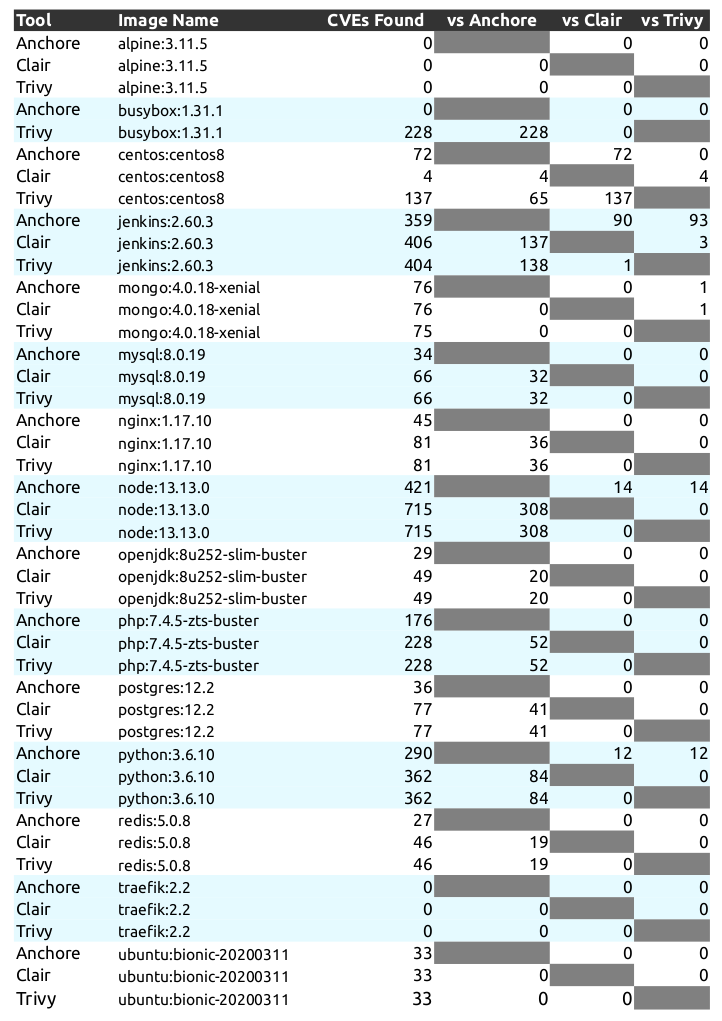
\includegraphics[scale=0.5]{graphics/Docker-Image-Static-Analysis-Tool-Comparison-Table.png}
    \caption{Comparison of Anchore Engine, Clair, and Trivy}
    \label{fig:docker_comparison}
\end{figure}

Some of the tool are easier to implement than others for the purpose of e.g. continuous integration, which is more or less the case for this thesis. Anchore Engine and Clair have to be deployed as a service and need to be accessible for the pipeline. In case of Kubernetes this isn't an issue, but it comes along with additional overhead as those tools were simply not developed as a target of CI. Anchore Engine in this case is better than Clair as it comes along with a ready to use CLI, while Clair requires one to use a third party implementation to interact with it. Triviy was built for the purpose of CI and can be integrated as another container in the Kubernetes pod, which then pulls the latest database filled with CVEs and runs the scan against the defined images in the pipeline, e.g. locally built images or images pulled from Docker registries.

\todo{CVSS}
\subsubsection{Calculation of Score}
\subsubsection{Orchestrator / Funnel}
\todo{Normalization}
\subsection{Frontend}
\subsubsection{Content-based Recommendation}
\section{Expandability}
\todo{current focus on docker-compose, but can easily be extended to further sources, may it be crawling/processing/analysing/showing}
\section{IaC of implementation}

%\section{Open Source}
%\subsection{GitHub}

%\section{Architecture}
%\subsection{Microservices}
%\subsection{Software design pattern}
%\todo{Strategy pattern}
%\todo{Singleton}
%\subsection{Node.js}
%\subsection{React}

%\section{Protocols}
%\subsection{WebSocket}
%\subsection{REST}
%\subsection{gRPC}
%\subsection{JNLP}